%------------------------------------------
%	$Id$
%
%	The GMT Documentation Project
%	Copyright (c) 2000-2012.
%	P. Wessel, W. H. F. Smith, R. Scharroo, J. Luis and F. Wobbe
%------------------------------------------
%
\chapter{Of colors and color legends}
\label{app:M}
\section{Built-in color palette tables}
\index{CPT!built-in set}
\index{color!palette tables}

Figure~\ref{fig:GMT_App_M_1} shows each of the 22 built-in color palettes,
stored in so-called CPT tables\footnote{The 23rd palette is called \emph{random}
and produces a random set of colors suitable for categorical plots.}.
The programs \GMTprog{makecpt} and \GMTprog{grd2cpt} are used to access these master CPT tables
and translate/scale them to fit the user's range of $z$-values.
The top half of the color bars in the Figure shows the original color scale, which can be either discrete or
continuous, though some (like \textbf{globe}) are a mix of the two.
The bottom half the color bar are built by using
\GMTprog{makecpt} \Opt{T-1/1/0.25}, thus splitting the color scale into 8 discrete colors.

\begin{figure}[h]
\centering

\includegraphics[width=\textwidth]{GMT_App_M_1}
\caption{The standard 22 CPT files supported by \gmt.}
\label{fig:GMT_App_M_1}
\end{figure}

\section{Labeled and non-equidistant color legends}
\label{app:colorbars}
\index{color!legend}
The use of color legends has already been introduced in Chapter~\ref{ch:7} (examples 2, 16, and 17). Things become a bit more complicated when you want to label the legend with names for certain intervals (like geological time periods in the example below). To accomplish that, one should add a semi-colon and the label name at the end of a line in the CPT table and add the \Opt{L} option to the \GMTprog{psscale} command that draws the color legend. This option also makes all intervals in the legend of equal length, even it the numerical values are not equally spaced.

Normally, the name labels are plotted at the lower end of the intervals. But by adding a \emph{gap} amount (even when zero) to the \Opt{L} option, they are centered. The example below also shows how to annotate ranges using \Opt{Li} (in which case no name labels should appear in the CPT file), and how to switch the color bar around (by using a negative length).

\script{GMT_App_M_2}

\begin{figure}[h]
\centering
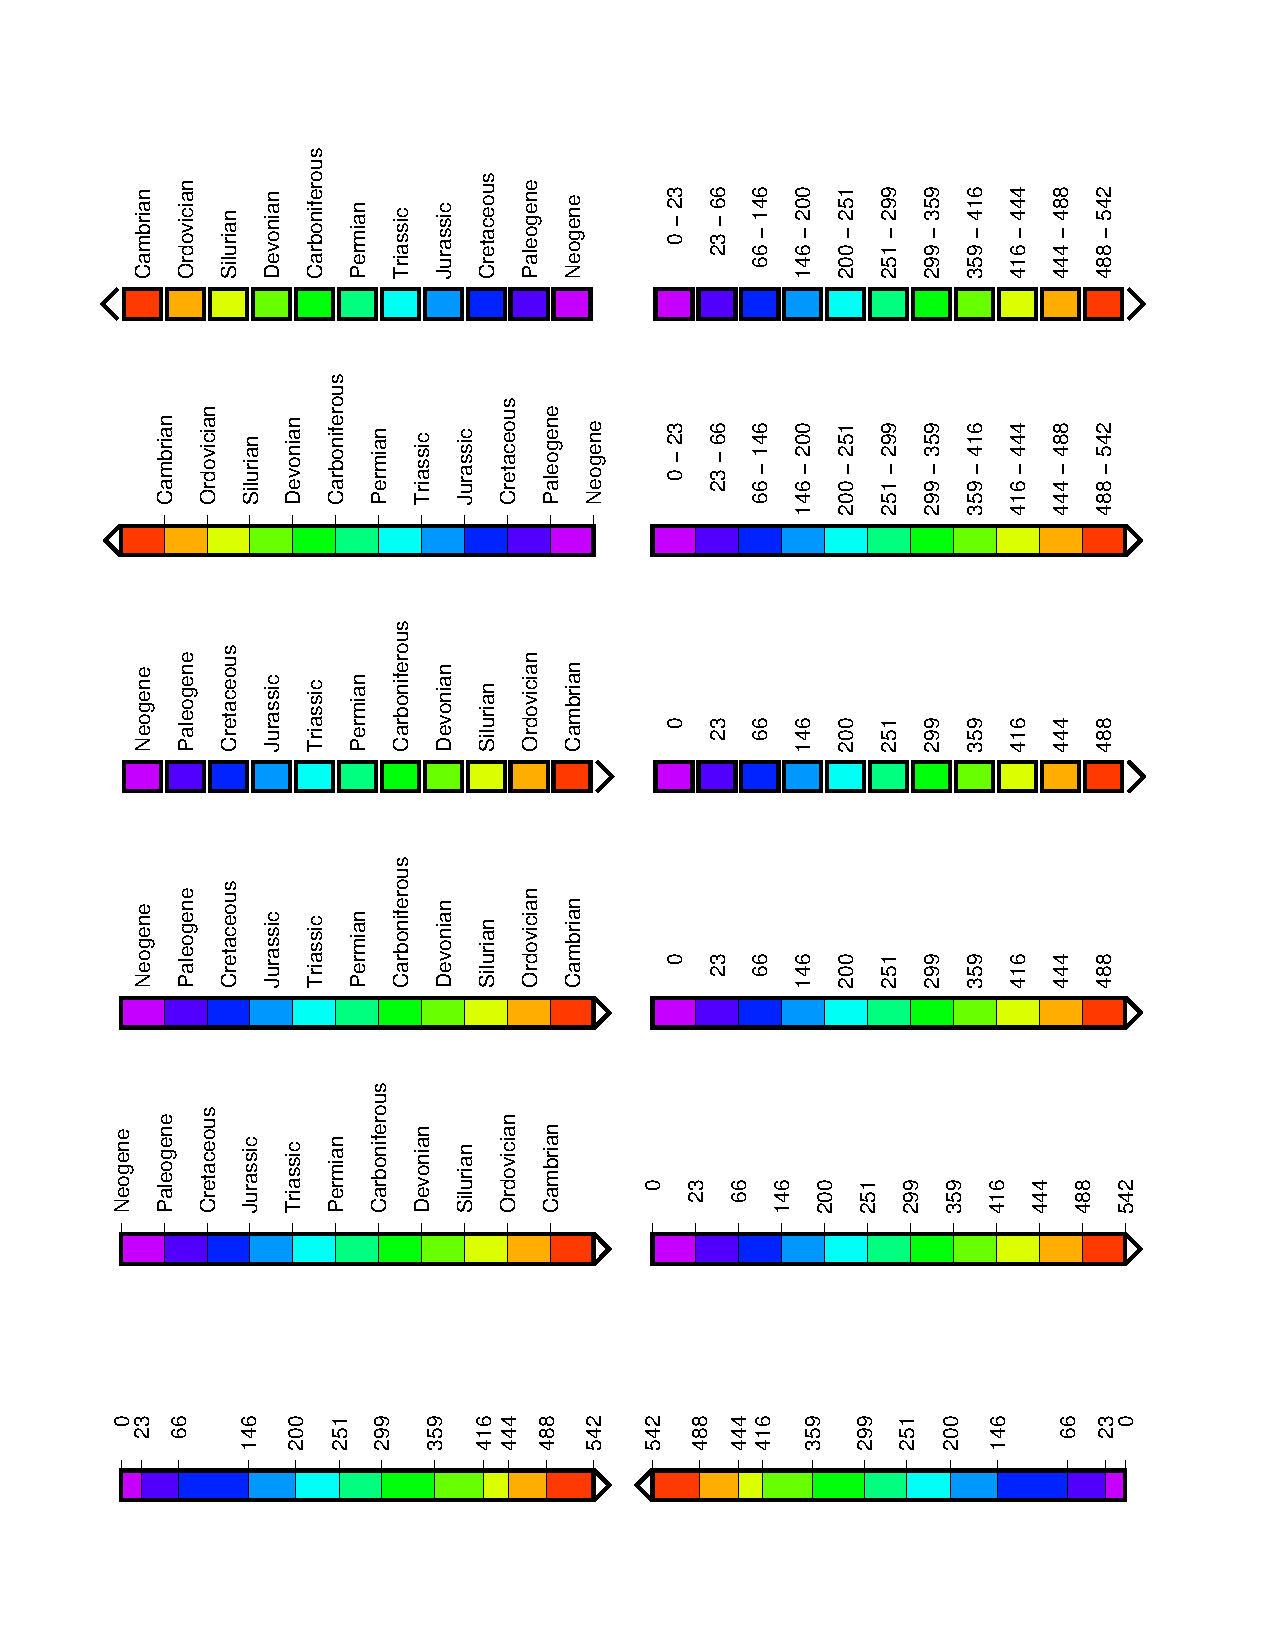
\includegraphics[width=\textwidth]{GMT_App_M_2}
\caption{The many forms of color legends created by \protect\GMTprog{psscale}.}
\label{fig:GMT_App_M_2}
\end{figure}
